\documentclass{article}

\usepackage{graphicx}
\usepackage{hyperref}

\title{User Interface Parsing \\ \small{Progress Update}}
\author{Calvin Loncaric}
\date{April 15, 2015}

\begin{document}

\maketitle

\noindent This project is off to a good start. \autoref{fig:screenshot} shows a
screenshot of the current tool, demonstrating line detection and grouping. Items
accomplished so far:
\begin{itemize}
\item Set up project structure, including linking to basic computer vision
    libraries (OpenCV for basic routines, Tesseract and Leptonica for character
    recognition).
\item Made scans of 14 hand-drawn sample interfaces. These will serve as the
    development set that I will test against during implementation. They
    have a wide range of features, including: strange layouts, text (both
    titles and paragraphs), images, floating images, distance constraints,
    and tabular data.
\item Implemented basic line recognition and grouping using the Hough
    transform.
\item Implemented line grouping using some custom heuristics: lines are grouped
    if they point in roughly the same direction and if their closest approach
    is less than some threshold.
\end{itemize}

\noindent My immediate next steps are:
\begin{itemize}
\item Improve line grouping. \autoref{fig:screenshot} clearly shows some lines
    being grouped together which do not belong together.
\item Start implementing high-level explanation: every line is part of text, a
    distance measurement, or a box (with other options to be added later).
    These high-level explanations will, in the long-term, be used to construct
    the actual layout.
\end{itemize}

\begin{figure}
    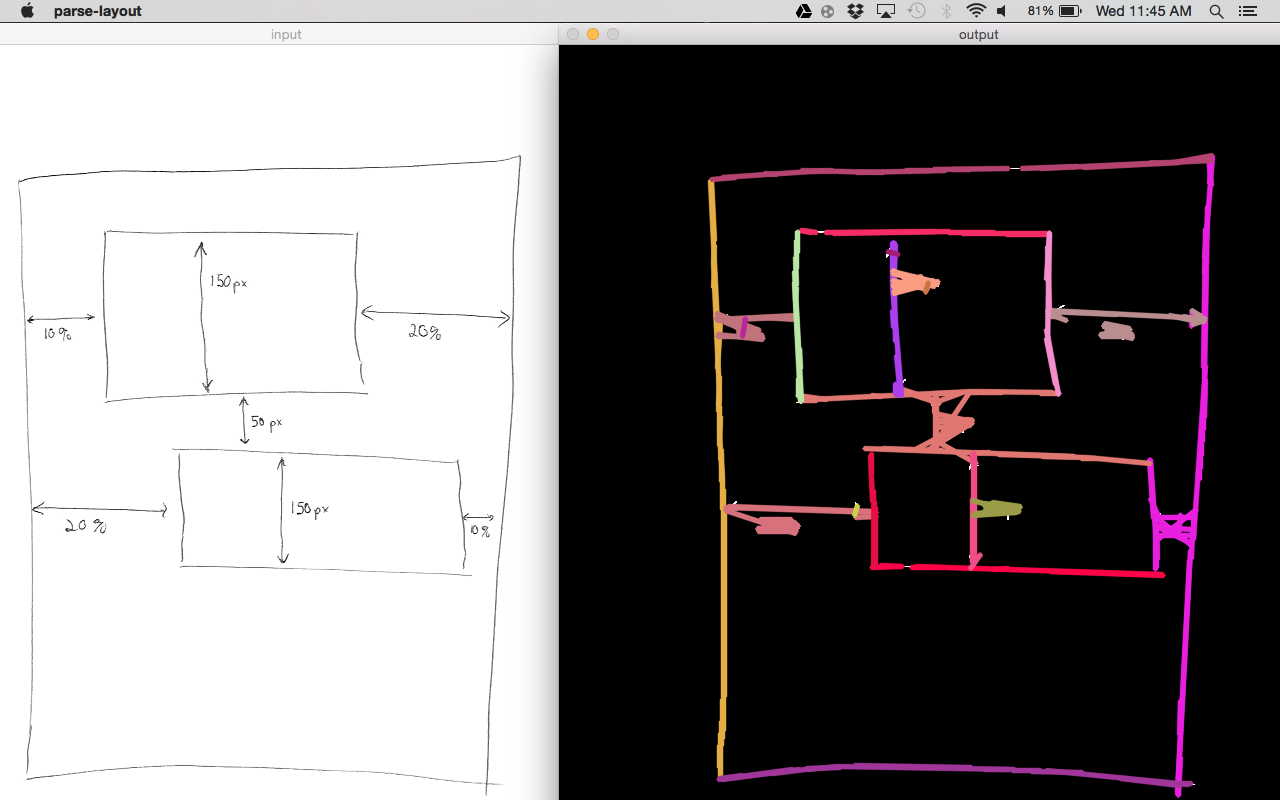
\includegraphics[width=\textwidth]{progress-2015-04-15-screenshot.png}
    \caption{Screenshot of the current tool demonstrating stroke recognition.
        Groups of lines are colored by which group they belong to.}
    \label{fig:screenshot}
\end{figure}

\end{document}
